\documentclass{article}

\usepackage{graphicx}
\graphicspath{ {./figs/} }

\title{Indoor Localization and Finding Optimal Path Using Image Processing and Machine Learning}
		 
\author{Mohamad Orabi, Elie Raad, \\Rita Mahfood, Kareem Abi Fadel}

\begin{document}
\maketitle
\pagebreak

\tableofcontents
\pagebreak

\section{Introduction}
Place Holder Text
\section{Constraints and Standards}
Place Holder Text

\section{Background}
To understand the relevance, impact, and importance of our project, we must first shed light on the importance of indoor localization as well as elaborate on why the most common solution GPS is not sufficient indoors.

\subsection{The need for indoor localization vs outdoor localization using GPS}
After GPS became freely accessible to the public in the 1980's, a huge amount of research was able to make this service extremely reliable, and made outdoor localization and navigation something most people take for granted. Nowadays, a lot of our most advanced technologies are heavily reliant on GPS for their operations. This is due to the incredible accuracy 1-3 meters that it can provide outdoors. Enhancements to this system such as differential GPS increase its accuracy to 1-3 centimeters, allowing it to be used in situations that are high in risk and require extreme precision such as airplane landing [Add reference here]. 
\newline
 
When most people think of localization and navigation, what they imagine is them being outdoors in an unfamiliar location and using their phones for navigation. This however is not because this problem is only relevant when they are outdoors, it is because this is what our society is exposed to. Nonetheless, the problem of indoor localization is growing more and more relevant as we continue to build huge structures such as shopping centers, malls, universities, parking structures, etc.

\subsection{Efficiency of GPS on indoor localization}
To understand the limitations of GPS localization indoors, we must have a basic understanding of how it operates. GPS is used by millions of people simultaneously worldwide. Hence, it is only logical that the signals transmitted by these satellites are passive and contain no information about the receiver. A GPS signal only contains information about the satellite itself, and a receiver then uses that information along with the distance traveled by the signal to determine its location. This method for determining position is called trilateration and is illustrated in figure \ref{trilateration}.
\newline

Therefore, a GPS's positioning accuracy is dependent on how accurately a receiver can measure the distance between it and the corresponding satellite known as pseudorange. A main source of error for GPS signals is multipath, which is when replicas of the original line of sight (LOS) signal bounce off of reflecting surface and to the input of the antenna. Multipath is a common issue for GPS both indoors and outdoors, but while multiple methods have been developed to accurately track the LOS signal and mitigate the effects of multipath outdoors [Add references here], in most cases the LOS signal is not visible when the receiver is indoors, and hence the receiver will not be able to produce a correct pseudorange measurement.


\begin{figure}[h!]
\centering
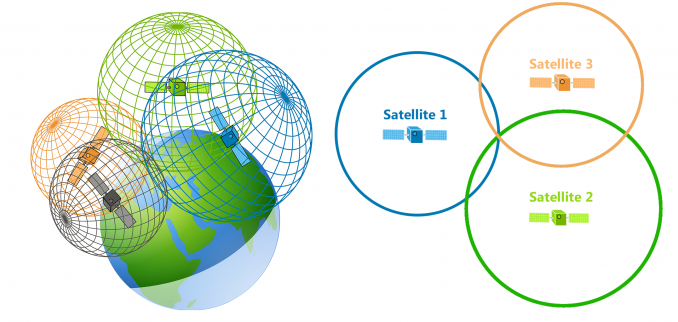
\includegraphics[width=8cm]{Trilateration}
\caption{\label{trilateration} Trilateration }
\end{figure}


\section{Solution and Expectations}
Place Holder Text

\subsection{Different ways of indoor localization}
Place Holder Text

\subsection{Applications of indoor localization}
Place Holder Text

\subsection{Use of indoor localization inside shops}
Place Holder Text

\section{Our Design}
Place Holder Text

\subsection{Software}
Place Holder Text

\subsection{Hardware}
Place Holder Text

\section{Conclusion}
Place Holder Text

\section{References}
Place Holder Text




\end{document}
